% !TEX TS-program = pdflatex
% !TEX encoding = UTF-8 Unicode
\documentclass[18pt,aspectratio=169]{beamer}
% Make the theme files in example_theme/ findable regardless of build tool
% (Texmaker, TeXShop, latexmk, ...) without needing TEXINPUTS/BIBINPUTS set.
\makeatletter
\def\input@path{{example_theme/}}
\makeatother
\graphicspath{{example_theme/}}
\setlength{\itemsep}{2pt}
\setlength{\parskip}{2pt}
\setbeamersize{text margin left=5mm, text margin right=5mm}

\usepackage[utf8]{inputenc}
\usepackage[T1]{fontenc}
\usepackage{listings}
\usepackage{physics}
\usepackage{arydshln}

\title{Toward Quantum Competitiveness in Adiabatic Quantum Computing: A Comparative Study of Variational and Factoring Algorithms}
\date{}
\author{Philipp Hanussek}
\institute{Master 2 Quantum Information, Sorbonne Universit\'e, Paris, France\\Supervisor: dr hab. Bart{\l}omiej Gardas, IITiS PAN, Gliwice, Poland}

% \usetheme[logo=medecine,style=medecine]{sorbonne} % pour un theme plus rouge et le logo médecine (par défaut)
% \usetheme[logo=universite,style=universite]{sorbonne} % pour un theme plus bleu foncé et le logo université
\usetheme[logo=sciences,style=sciences]{sorbonne} % pour un theme plus bleu clair et le logo sciences
% \usetheme[logo=lettres,style=lettres]{sorbonne} % pour un theme plus jaune et le logo lettres
% logo et theme sont mixables
% \usetheme[logo=medecine,style=universite]{sorbonne} % pour un theme plus rouge et le logo médecine
\usetikzlibrary{shapes.geometric,calc}

% biblatex would need texlive-bibtexextra; use plain bibtex (as report.tex does) instead.
\usepackage{natbib}
\bibliographystyle{unsrt}

\begin{document}

\begin{frame}[plain]
\titlepage
\begin{tikzpicture}[remember picture, overlay]
    % placed to sit immediately left of the theme's auto-inserted Sorbonne
    % logo (anchor south east, xshift=-0.5cm, yshift=0.5cm, width=2.5cm)
    \node[anchor=south east, xshift=-3.4cm, yshift=0.5cm, fill=white, rounded corners=2pt, inner sep=2pt] at (current page.south east) {
\includegraphics[height=1cm]{../figures/logo/iitislogo.png}};
\end{tikzpicture}
\end{frame}

\begin{frame}
        \frametitle{Sommaire}
        \tableofcontents
        %\tableofcontents[hideallsubsections]
\end{frame}

\section{Local Context}

\begin{frame}{Local Context}
\begin{columns}[T,onlytextwidth]
\begin{column}{0.42\textwidth}
\begin{itemize}
    \item Institute of Applied and Theoretical Informatics, Polish Academy of Sciences
    \item Quantum Systems for Informatics group
    \item Work on Adiabatic Quantum Computing, simulation of many-body quantum systems
\end{itemize}
\end{column}
\begin{column}{0.58\textwidth}
\centering
% Poland_adm_location_map.pdf is rsvg-convert'd from Poland_adm_location_map.svg
% (pdflatex cannot include SVG directly); viewBox 861.39 x 837.239,
% Gliwice at 50.294N 18.666E within map bounds top=55.2 bottom=48.7 left=13.8 right=24.5
% (Wikipedia Module:Location_map/data/Poland), giving fractional position (0.4548, 0.7547).
\begin{tikzpicture}
    \def\PolandWcm{6.2}
    \pgfmathsetmacro{\PolandHcm}{\PolandWcm*0.97196}
    \pgfmathsetmacro{\GliwiceXcm}{\PolandWcm*0.4548}
    \pgfmathsetmacro{\GliwiceYcm}{\PolandHcm*0.7547}
    \node[anchor=north west, inner sep=0pt] (map) at (0,0) {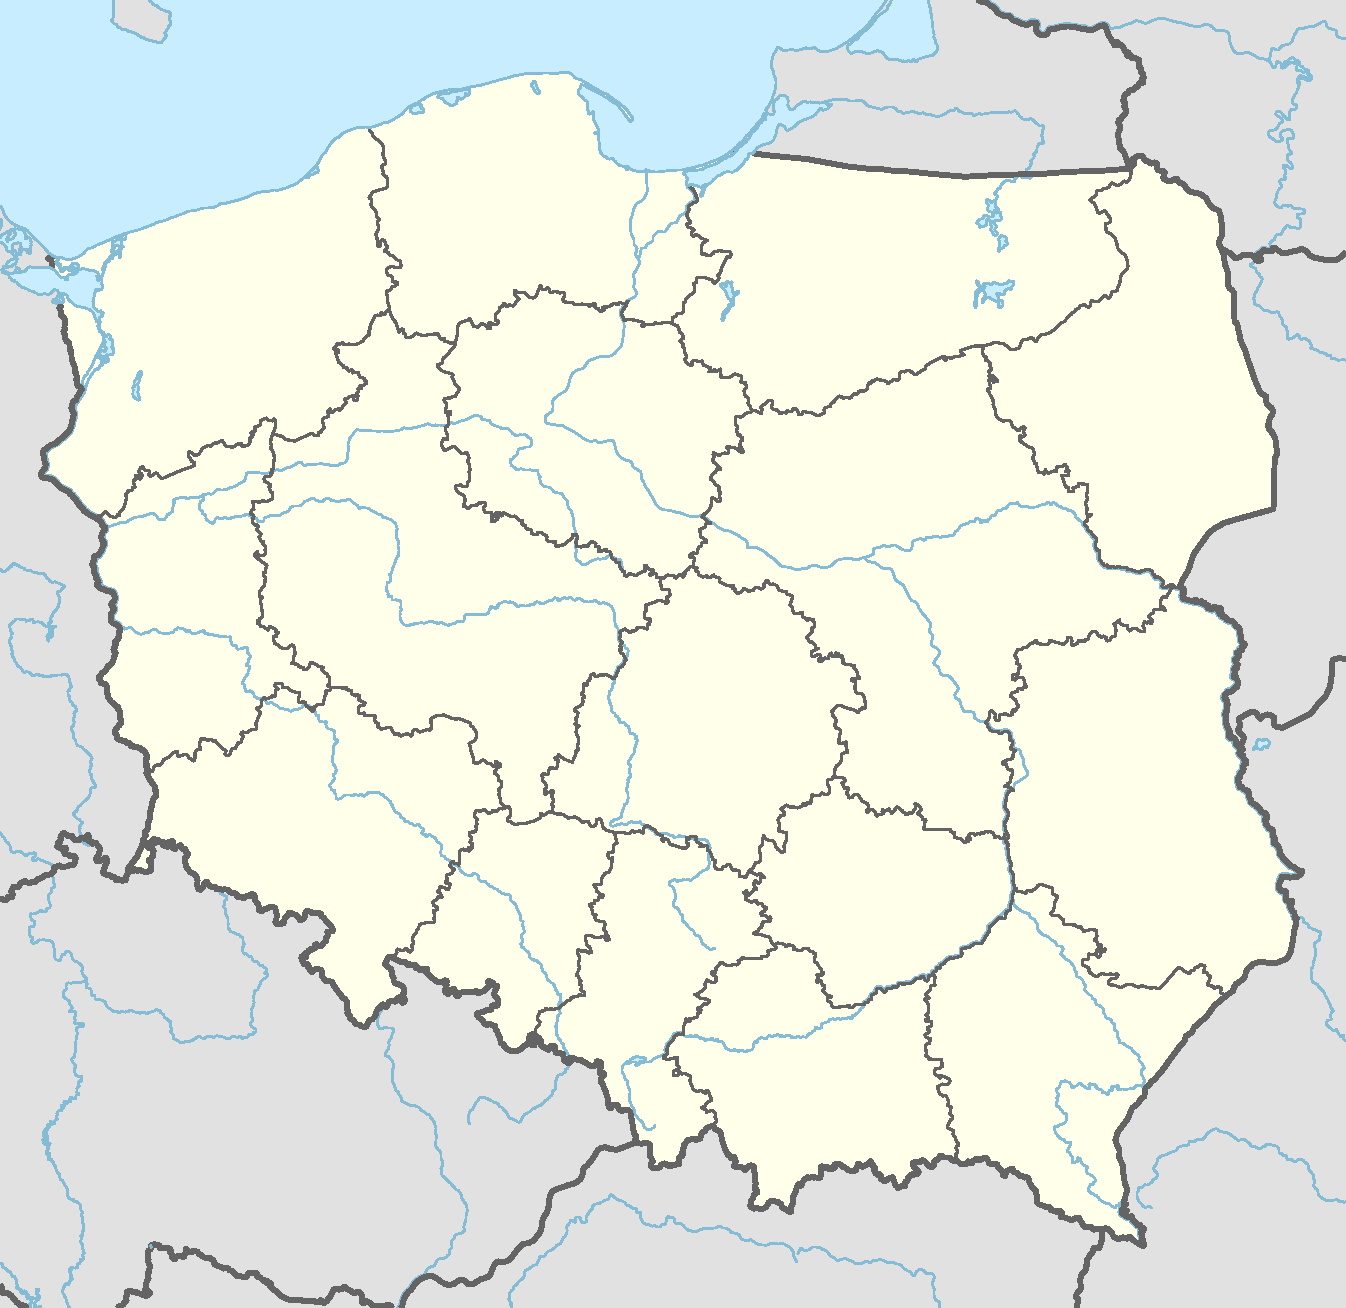
\includegraphics[width=\PolandWcm cm]{../figures/Poland_adm_location_map.pdf}};
    \coordinate (gliwice) at ($(map.north west) + (\GliwiceXcm cm, -\GliwiceYcm cm)$);
    \node[star, star points=5, star point ratio=2.25, fill=orange, draw=black, thin, minimum size=0.4cm, inner sep=0pt] at (gliwice) {};
    \node[fill=white, draw=black, thin, rounded corners=1pt, inner sep=2pt, font=\scriptsize\bfseries, anchor=west, xshift=3mm] at (gliwice) {Gliwice};
\end{tikzpicture}
\end{column}
\end{columns}
\end{frame}

\begin{frame}{Previous work}
\begin{itemize}
    \item Previous results on \textit{exact solving} were not very promising
    \item Problems where a wide range of samples, not necessarily the exact solution, can be exploited
\end{itemize}

\vfill

\begin{columns}[T,onlytextwidth]
\begin{column}{0.48\textwidth}
    \centering
    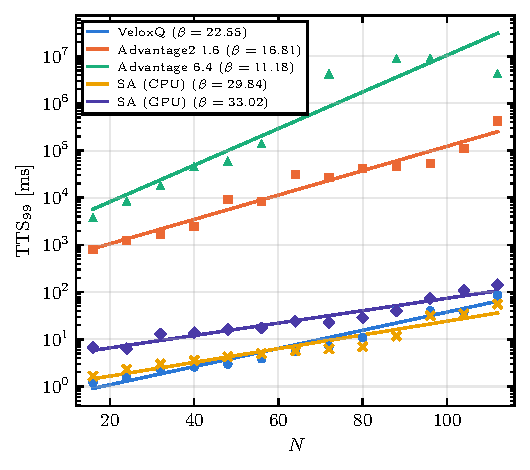
\includegraphics[height=3.9cm]{../figures/tta_overview_native.pdf}\\
    \footnotesize (a) Time-to-success, quantum simulation\\
    {\tiny doi:10.1103/rrf3-jm5m}
\end{column}
\begin{column}{0.48\textwidth}
    \centering
    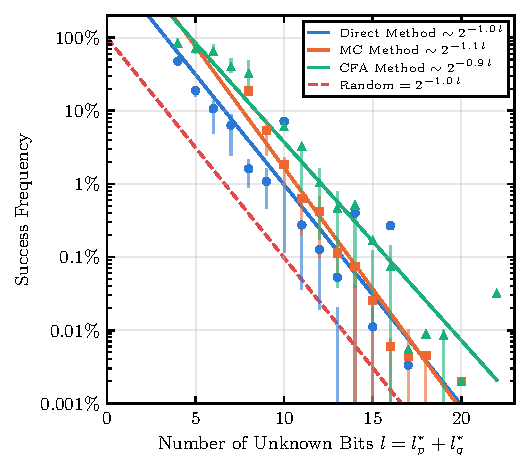
\includegraphics[height=3.9cm]{../figures/factoring_success.pdf}\\
    \footnotesize (b) Success rate prime factorization\\
    {\tiny arXiv:2410.14397}
\end{column}
\end{columns}
\end{frame}


\section{Quantum Annealing}

\begin{frame}{D-Wave Quantum Annealer}
\begin{columns}[T,onlytextwidth]
\begin{column}{0.56\textwidth}
\footnotesize
\begin{block}{Driver Hamiltonian}
\begin{equation*}
H_D=-\sum_{i=1}^N \sigma_x^{(i)} \text{ with ground state } \ket{+}^{\otimes N}
\end{equation*}
\end{block}
\begin{block}{Problem Hamiltonian}
\begin{equation*}
H_P=\sum_{i=1}^N h_i\sigma_z^{(i)}+\sum_{i=1}^N\sum_{j=1}^{i-1} J_{ij}\sigma_z^{(i)}\otimes\sigma_z^{(j)}
\end{equation*}
\end{block}

\begin{alertblock}{}
Stays in the ground state according to the adiabatic theorem~\cite{Born_Fock_1928,Farhi_2000}
\end{alertblock}
\end{column}
\begin{column}{0.4\textwidth}
    \centering
    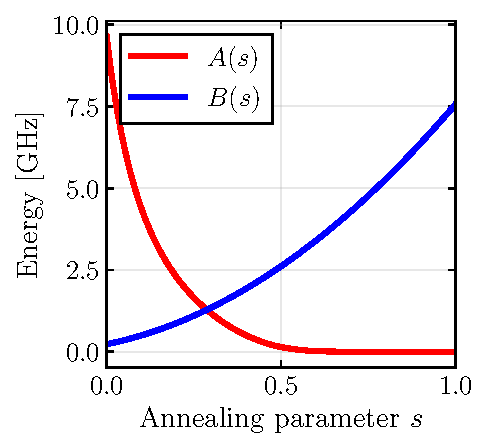
\includegraphics[width=\linewidth]{../figures/anneal_schedule_plot.pdf}\\
    \footnotesize Annealing schedules $A(s)$, $B(s)$
\end{column}
\end{columns}
\end{frame}

\begin{frame}{D-Wave Connectivity}
\begin{columns}[T,onlytextwidth]
\begin{column}{0.48\textwidth}
    \centering
    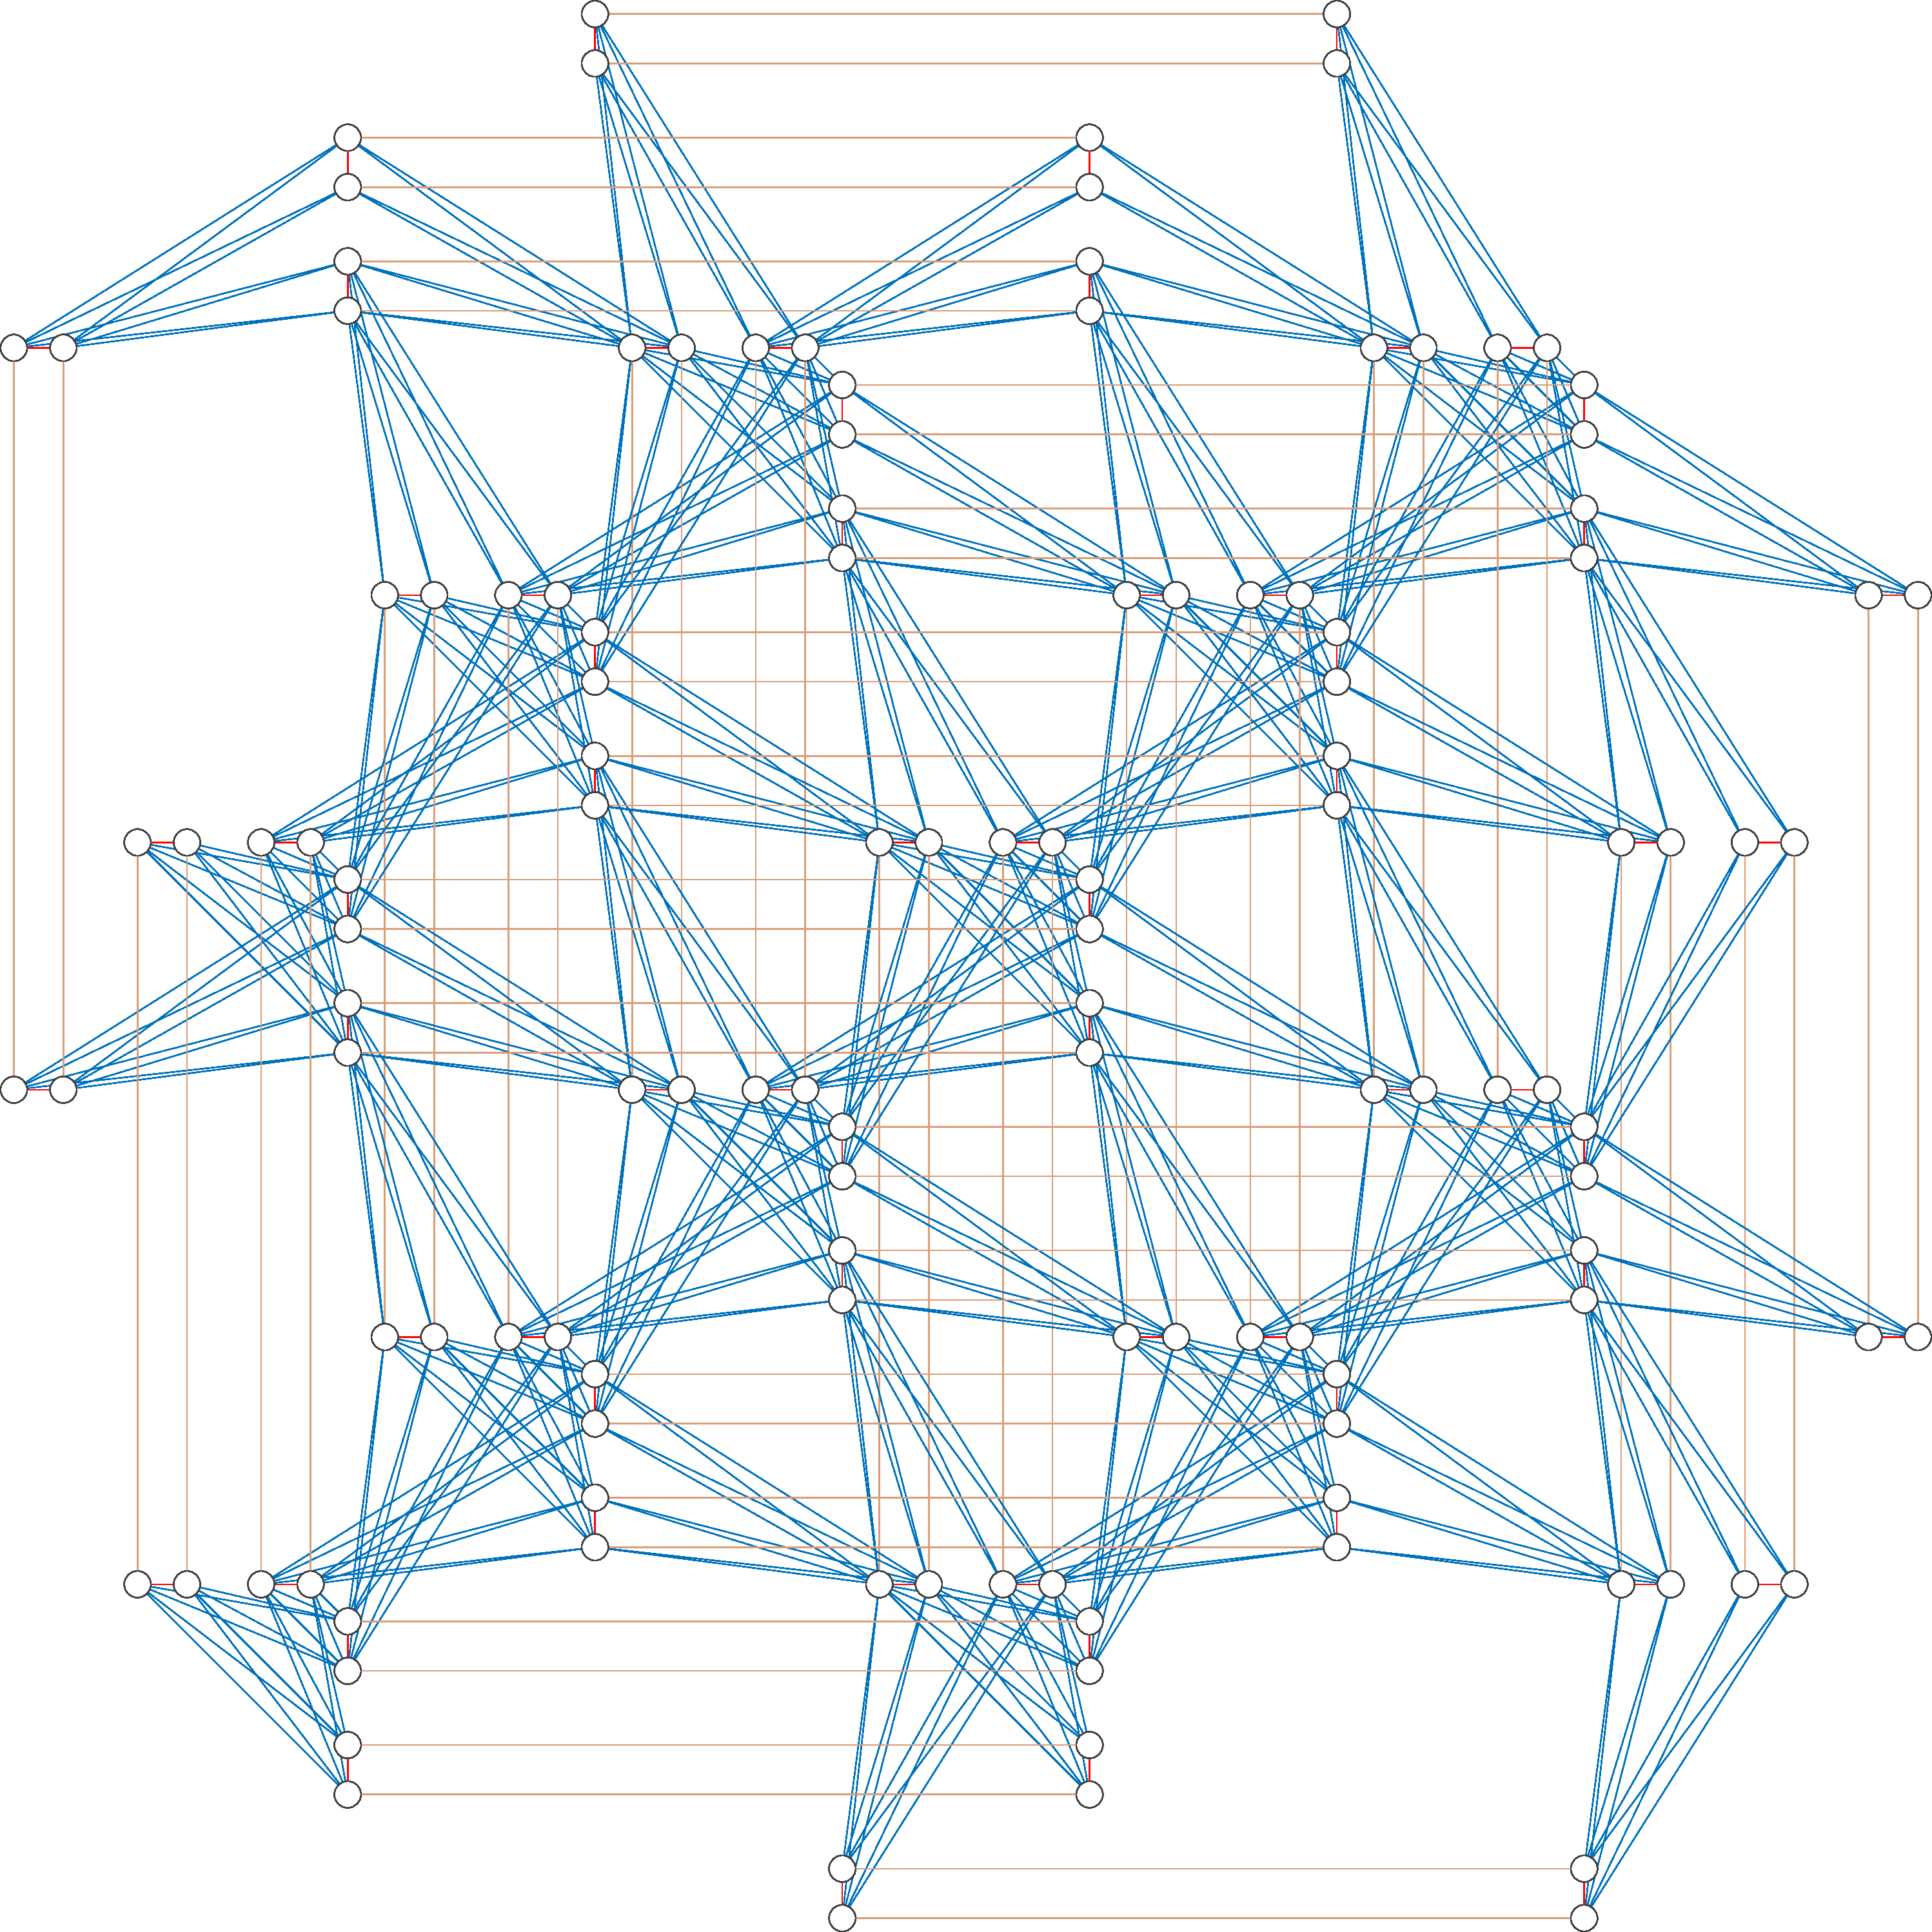
\includegraphics[height=5cm]{../figures/pegasus.pdf}\\
    \footnotesize (a) Pegasus (Advantage)
\end{column}
\begin{column}{0.48\textwidth}
    \centering
    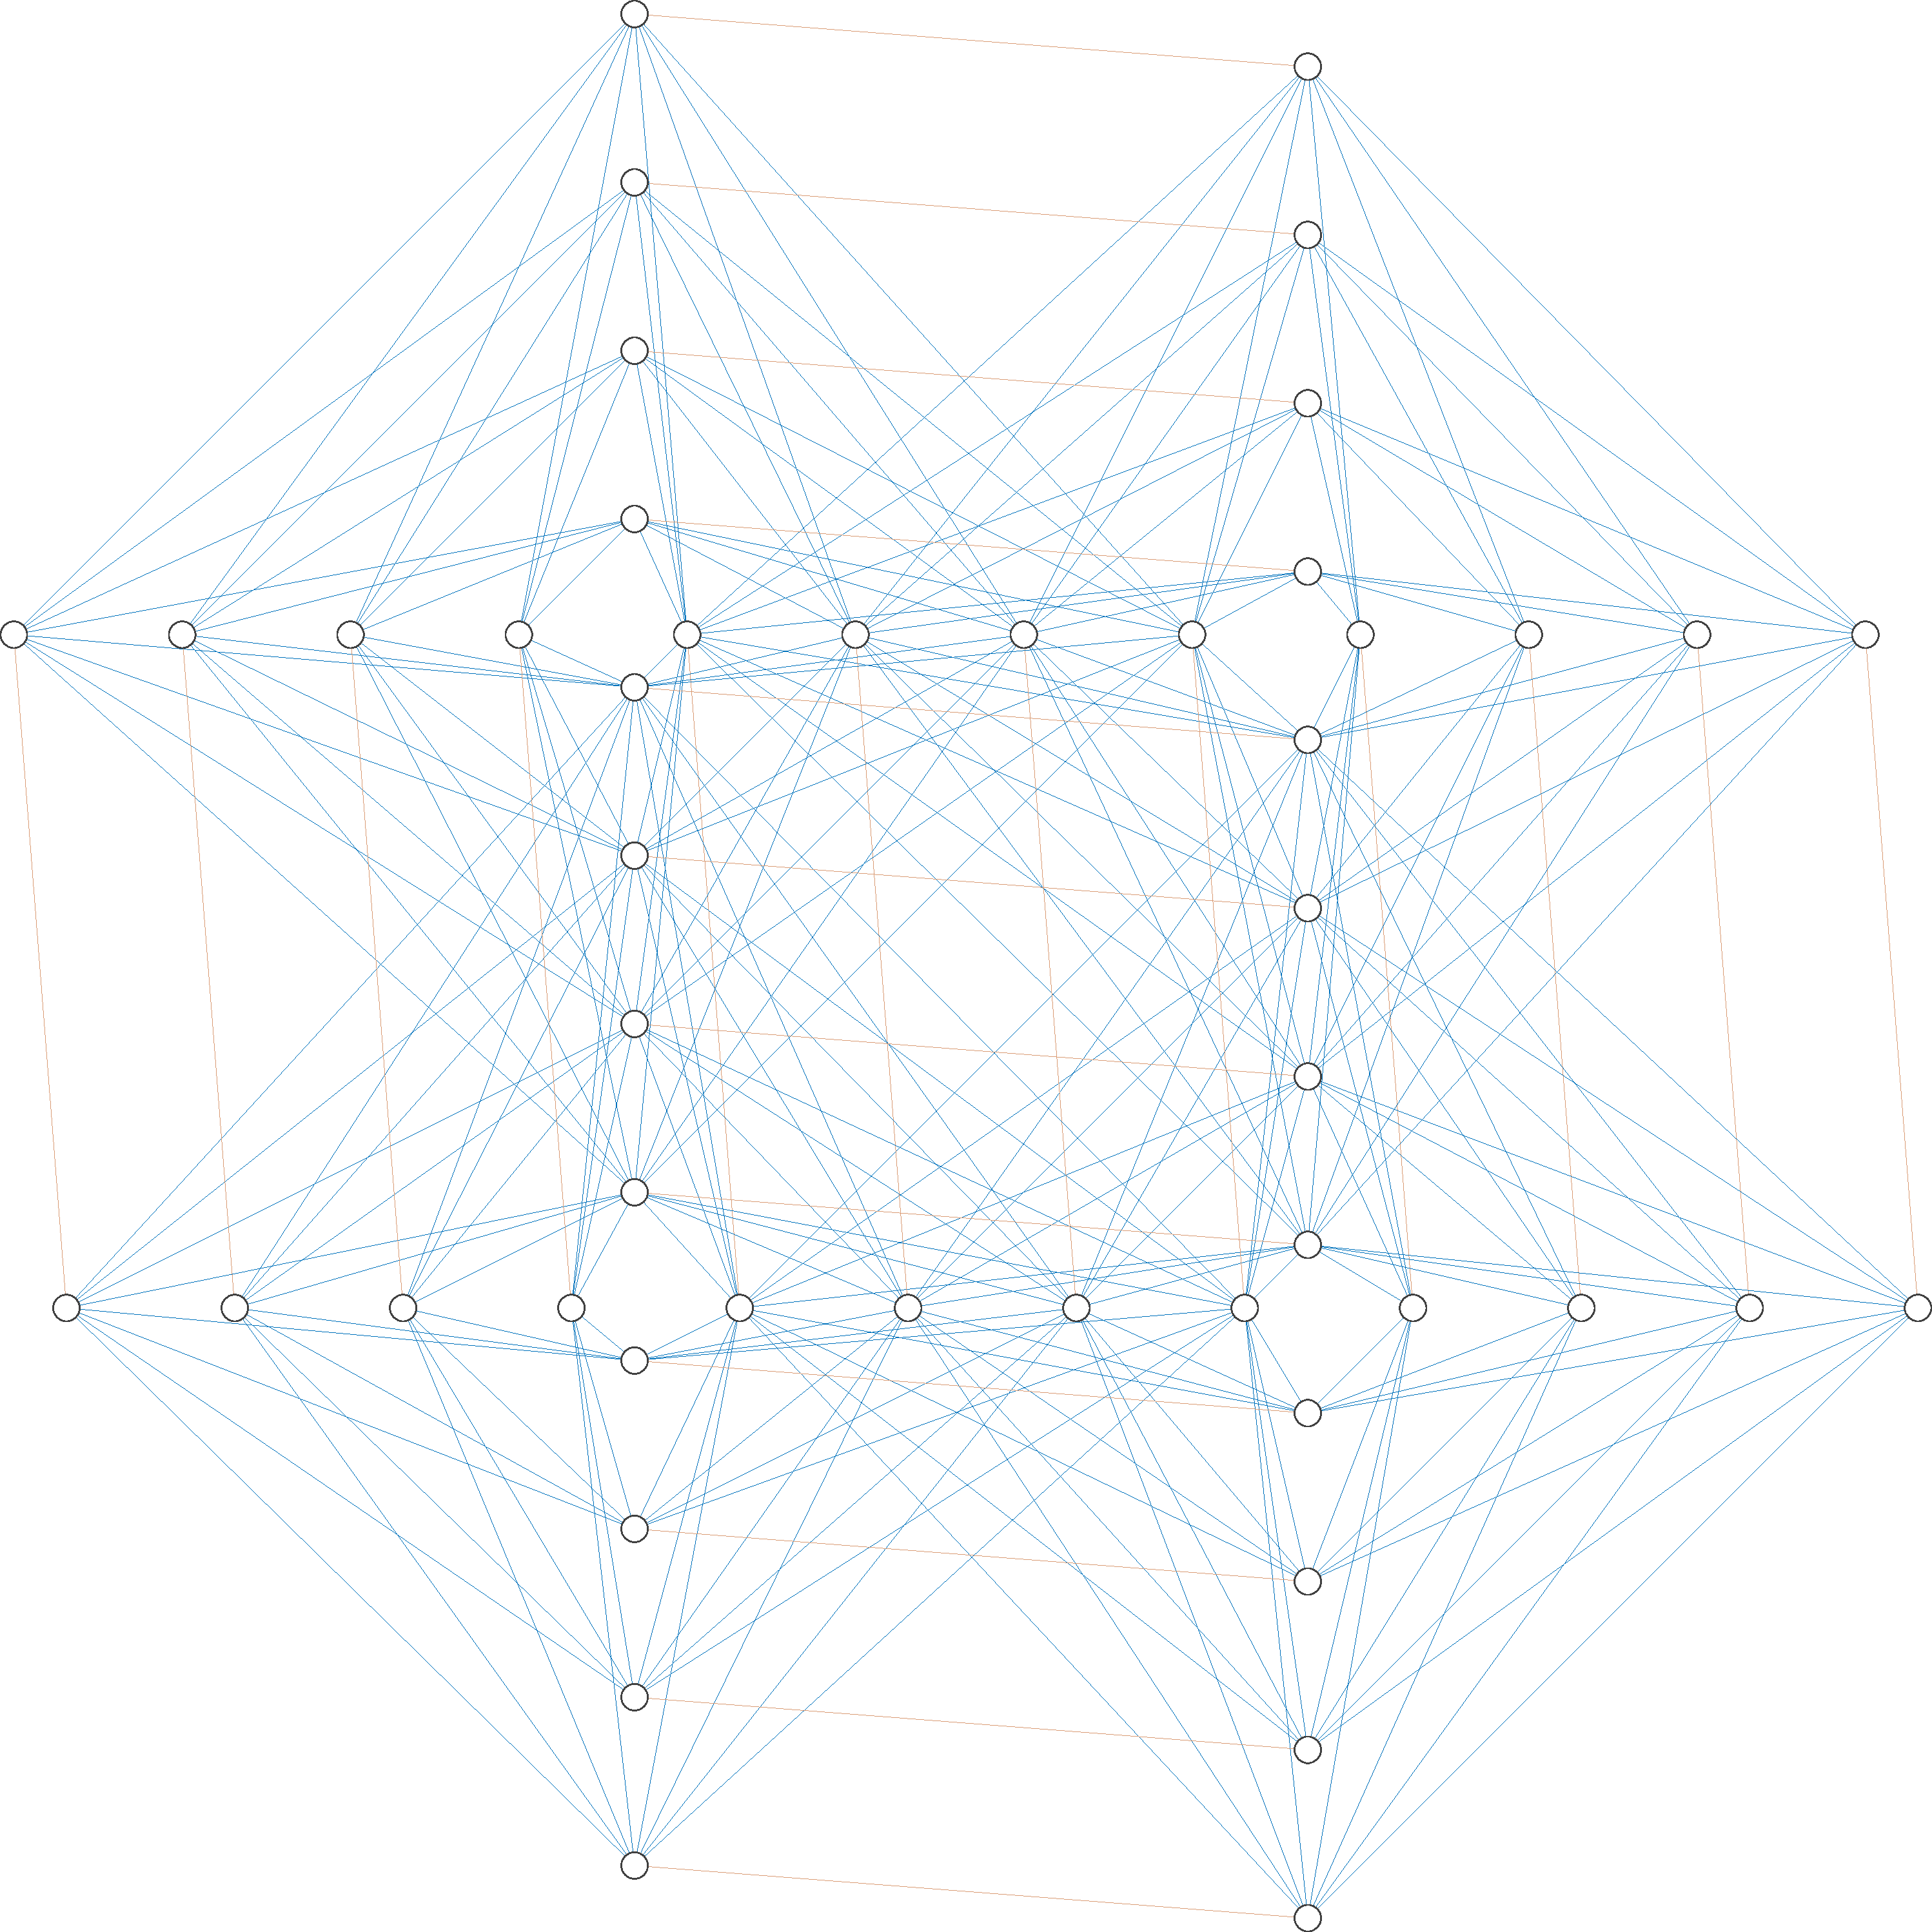
\includegraphics[height=5cm]{../figures/zephyr.pdf}\\
    \footnotesize (b) Zephyr (Advantage2)
\end{column}
\end{columns}

\vfill
\centering
\footnotesize Circles: qubits; blue: internal couplers; orange: external couplers.\\
Zephyr has more couplers per qubit and longer-range links.
\end{frame}

\section{Factoring Problem}

\begin{frame}{Factoring Problem}
\begin{block}{Definition}
Given a composite integer $N$, find its non-trivial factors $p$ and $q$ such that
\begin{equation*}
N = p \times q
\end{equation*}
\end{block}

\vspace{1em}
\textbf{Methods}
\begin{itemize}
    \item Modified multiplication table method --- Jiang et al., 2018~\cite{Jiang_2018}
    \item Controlled full-adder (CFA) method --- Ding et al., 2023~\cite{Ding_2023}
\end{itemize}

\vfill
\footnotesize Based on my bachelor's thesis~\cite{Hanussek_2024_BSc}; see also~\cite{willsch2024state}
\end{frame}

\begin{frame}{Modified Multiplication Table Method}
\centering
\footnotesize
\renewcommand{\arraystretch}{0.9}
\setlength{\tabcolsep}{4pt}
\begin{columns}[T,onlytextwidth]
\begin{column}{0.48\textwidth}
\centering
\begin{tabular}{c|ccccccc|}
 & $2^6$ & $2^5$ & $2^4$ & $2^3$ & $2^2$ & $2^1$ & $2^0$\\
\hline
$p$ & & & & & $1$ & $p_0$ & $1$\\
$q$ & & & & $1$ & $q_1$ & $q_0$ & $1$\\
\hline
 & & & & & $1$ & $p_0$ & $1$\\
$+$ & & & & $q_0$ & $p_0q_0$ & $q_0$ & \\
$+$ & & & $q_1$ & $p_0q_1$ & $q_1$ & & \\
$+$ & & $1$ & $p_0$ & $1$ & & & \\
\cdashline{1-6}
$+$ & & & & & $c_0$ & & \\
$+$ & & & $c_2$ & $c_1$ & & & \\
$+$ & & $c_4$ & $c_3$ & & & & \\
$+$ & $c_6$ & $c_5$ & & & & & \\
$+$ & $c_7$ & & & & & & \\
\hline
$N$ & $1$ & $0$ & $1$ & $1$ & $0$ & $1$ & $1$\\
\hline
\end{tabular}\\[2pt]
(a) Block size 1: 8 carry bits
\end{column}
\begin{column}{0.48\textwidth}
\centering
\begin{tabular}{c|cc|cc|cc|c|}
 & $2^6$ & $2^5$ & $2^4$ & $2^3$ & $2^2$ & $2^1$ & $2^0$\\
\hline
$p$ & & & & & $1$ & $p_0$ & $1$\\
$q$ & & & & $1$ & $q_1$ & $q_0$ & $1$\\
\hline
 & & & & & $1$ & $p_0$ & $1$\\
$+$ & & & & $q_0$ & $p_0q_0$ & $q_0$ & \\
$+$ & & & $q_1$ & $p_0q_1$ & $q_1$ & & \\
$+$ & & $1$ & $p_0$ & $1$ & & & \\
\hdashline
$+$ & & & $c_1$ & $c_0$ & & & \\
$+$ & $c_3$ & $c_2$ & & & & & \\
 & & & & & & & \\
 & & & & & & & \\
 & & & & & & & \\
\hline
$N$ & $1$ & $0$ & $1$ & $1$ & $0$ & $1$ & $1$\\
\hline
\end{tabular}\\[2pt]
(b) Block size 2: 4 carry bits
\end{column}
\end{columns}

\vfill
\footnotesize $3\times4$-bit multiplication table for $N=(1011011)_2=91$~\cite{Hanussek_2024_BSc,Jiang_2018}
\end{frame}

\begin{frame}{Modified Multiplication Table Method}
\small
From block size 2 (b) we obtain one equation per block:
\begin{align*}
2\bigl(1 + p_0q_0 + q_1 - (4c_1 + 2c_0)\bigr) + p_0 + q_0 &= (01)_2 = 1\\
2\bigl(q_1 + p_0 + c_1 - (4c_3 + 2c_2)\bigr) + q_0 + p_0q_1 + 1 + c_0 &= (11)_2 = 3\\
2c_3 + 1 + c_2 &= (10)_2 = 2
\end{align*}

\begin{block}{Cost function}
\begin{equation*}
f(p,q,c) = \sum_k \bigl(\text{LHS}_k - \text{RHS}_k\bigr)^2, \qquad \min f = 0 \iff N = p \times q
\end{equation*}
\end{block}
\vspace{-0.5em}
\begin{itemize}
    \item \textbf{Reduce:} higher-order terms (e.g.\ $p_0q_0\cdot p_0q_1$) to quadratic via auxiliary qubits
\end{itemize}

\vfill
\footnotesize Source:~\cite{Hanussek_2024_BSc,Jiang_2018}
\end{frame}

\begin{frame}{Controlled Full-Adder (CFA) Method}
\begin{columns}[c,onlytextwidth]
\begin{column}{0.58\textwidth}
\begin{block}{CFA gate}
\begin{equation*}
2\,c_\text{out} + \text{out} = (\text{enable} \land \text{in}_1) + \text{in}_2 + c_\text{in}
\end{equation*}
\end{block}

\vspace{0.5em}
\centering
\footnotesize
\renewcommand{\arraystretch}{1.05}
\setlength{\tabcolsep}{3pt}
\begin{tabular}{cccccccc}
\hline
 & & & & $p_2$ & $p_1$ & $p_0$ & $*q_0$\\
\hline
 & & & $N_{03}$ & $N_{02}$ & $N_{01}$ & $N_{00}$ & $+$\\
 & & & $p_2$ & $p_1$ & $p_0$ & & $*q_1$\\
\hline
 & & $N_{14}$ & $N_{13}$ & $N_{12}$ & $N_{11}$ & & $+$\\
 & & $p_2$ & $p_1$ & $p_0$ & & & $*q_2$\\
\hline
 & $N_{25}$ & $N_{24}$ & $N_{23}$ & $N_{22}$ & & & $+$\\
 & $p_2$ & $p_1$ & $p_0$ & & & & $*q_3$\\
\hline
$N_{36}$ & $N_{35}$ & $N_{34}$ & $N_{33}$ & & & & \\
\hline
\end{tabular}
\end{column}
\begin{column}{0.38\textwidth}
\centering
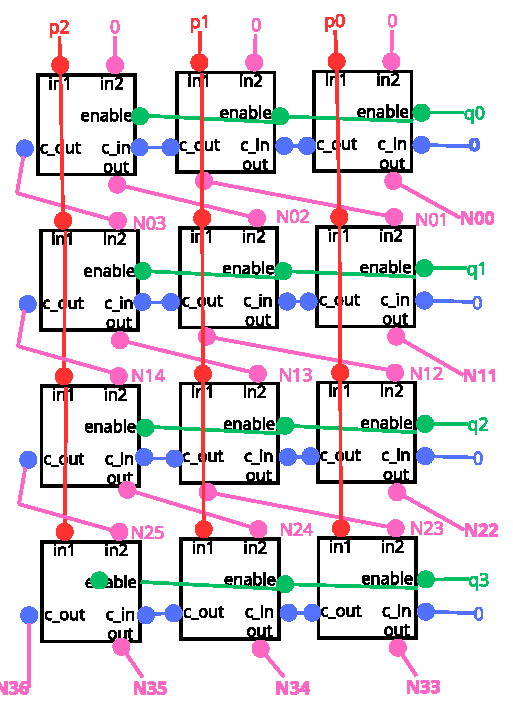
\includegraphics[height=6.3cm]{figures/cfa_multiplier_3x4.pdf}
\end{column}
\end{columns}

\vfill
\footnotesize Implementation of a $3\times4$-bit multiplier with CFAs~\cite[p.~5]{Ding_2023}; see~\cite{Hanussek_2024_BSc}
\end{frame}

\begin{frame}{CFA Method on the QPU}
\begin{columns}[c,onlytextwidth]
\begin{column}{0.45\textwidth}
\centering
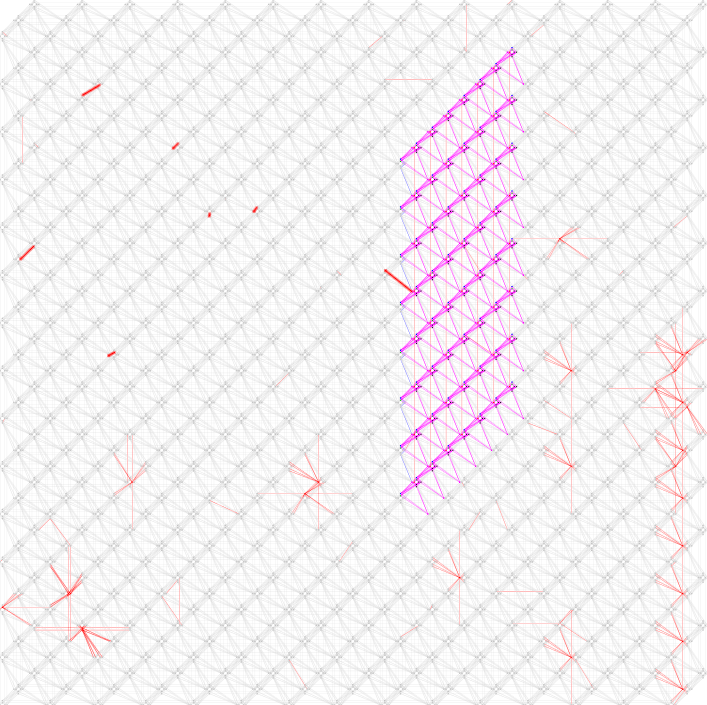
\includegraphics[height=5.6cm]{figures/cfa_qpu_adv54_7x8.png}\\
\footnotesize Advantage 5.4 QPU: $7\times8$-bit multiplier
\end{column}
\begin{column}{0.52\textwidth}
\begin{itemize}
    \item \textit{direct} into the hardware graph
    \item One CFA per unit cell 
\end{itemize}
\end{column}
\end{columns}

\vfill
\footnotesize Source:~\cite{Hanussek_2024_BSc,Ding_2023}
\end{frame}
\begin{frame}{Factoring Results}
\centering
\includegraphics[height=6.8cm]{../figures/factoring_results.pdf}

\vfill
\raggedright
\footnotesize Top: success frequency~\cite{willsch2024state}. Bottom: runs with ground state in samples~\cite{Hanussek_2024_BSc}
\end{frame}

\section{Quantum Ising Models}

\begin{frame}{Quantum Ising Model}
\begin{block}{TFIM Hamiltonian~\cite{mpg}}
\begin{equation*}
H=-J\sum_i\sigma_i^z\sigma_{i+1}^z-h\sum_i\sigma_i^x
\end{equation*}
\end{block}
\begin{itemize}
    \item we already saw something similar earlier ;)
\end{itemize}

\vfill
\centering
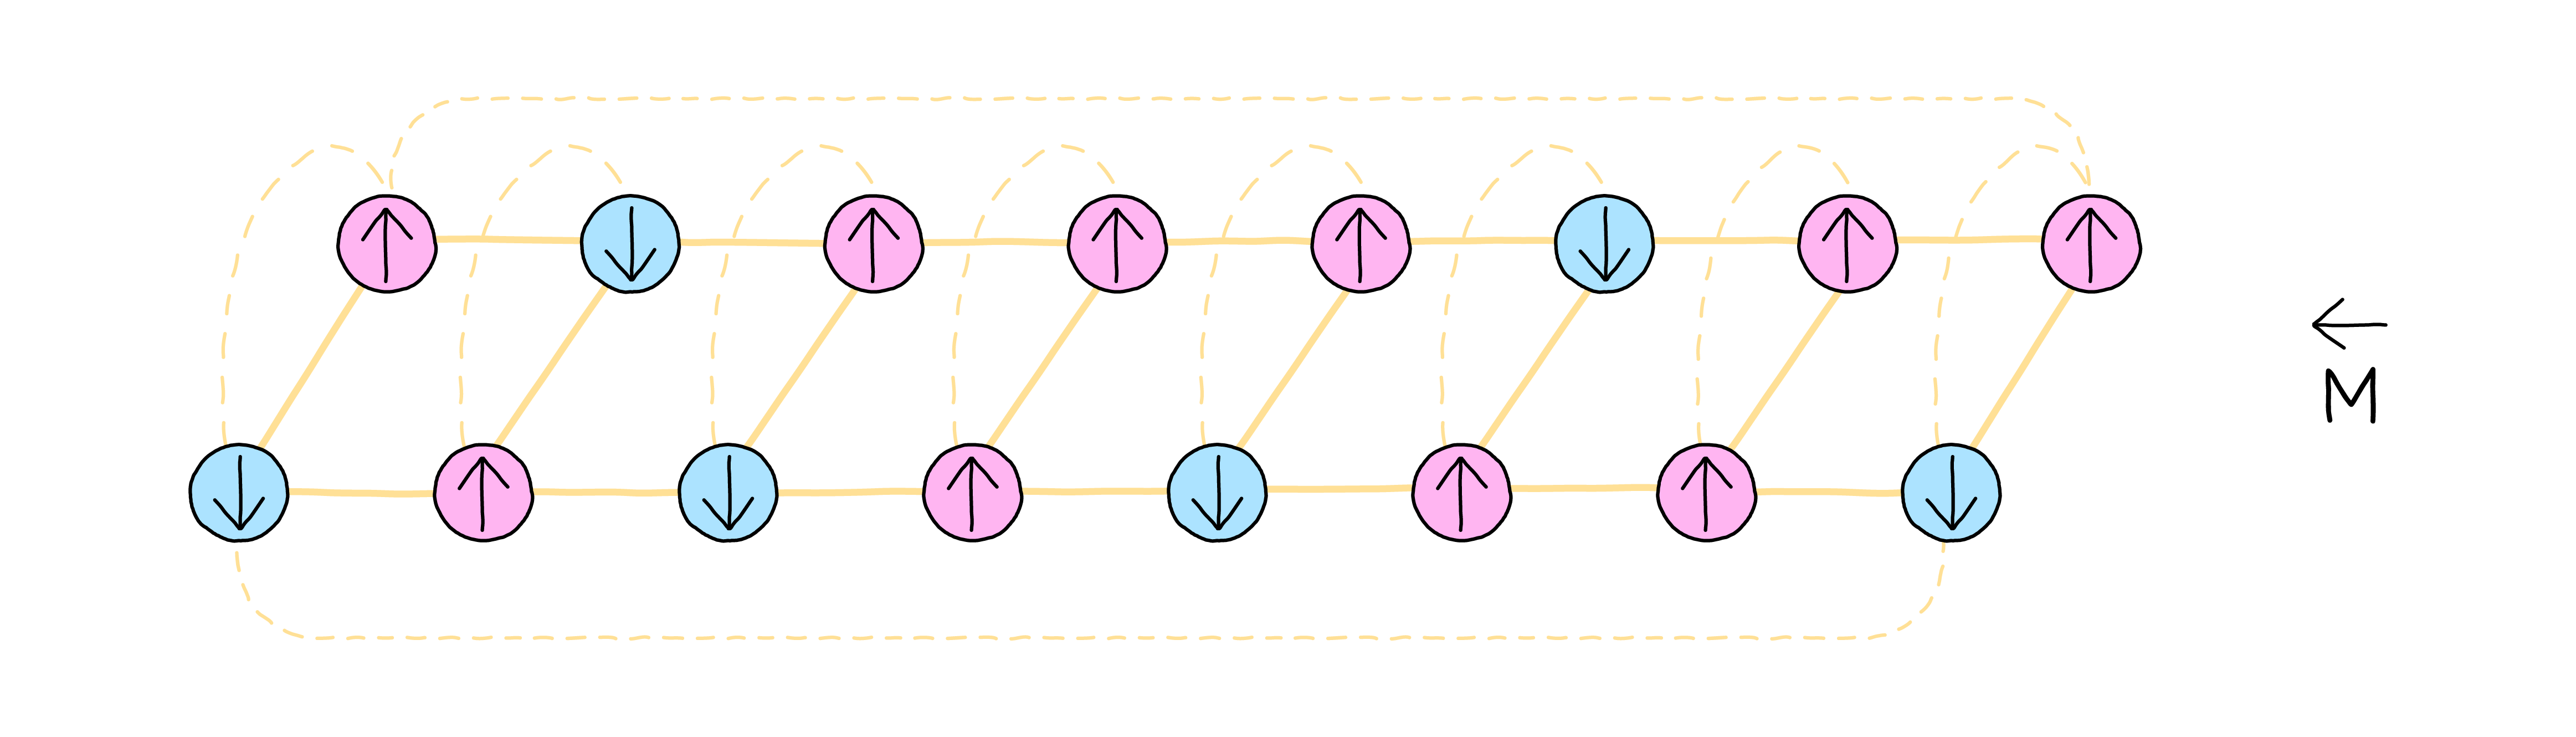
\includegraphics[width=0.75\linewidth]{figures/pennylane-datasets-hero-transverse-field-ising-model-a6af9251bad913ac2741c3f82019b38197417aa2.png}\\
{\scriptsize Image: PennyLane Datasets, \url{https://pennylane.ai/datasets/transverse-field-ising-model}}
\end{frame}

\begin{frame}{Heisenberg model (XXX)}
\begin{block}{Heisenberg Hamiltonian~\cite{Heisenberg_1928}}
\begin{equation*}
H = J_1 \sum_{i} \boldsymbol{\sigma}_i \cdot \boldsymbol{\sigma}_{i+1} + J_2 \sum_{i} \boldsymbol{\sigma}_i \cdot \boldsymbol{\sigma}_{i+2}
\end{equation*}
\footnotesize $\boldsymbol\sigma_i = (\sigma_i^x,\sigma_i^y,\sigma_i^z)$, so $\boldsymbol\sigma_i\cdot\boldsymbol\sigma_j = \sigma_i^x\sigma_j^x+\sigma_i^y\sigma_j^y+\sigma_i^z\sigma_j^z$
\end{block}
\begin{itemize}
    \item main difference to Ising: spin exchange instead of flipping, next nearest neighbor coupling
    \item goal in both cases: finding the \textbf{ground state} (and sampling from it)
\end{itemize}
\end{frame}

\begin{frame}{Example model: Ground state}
\begin{block}{TFIM Hamiltonian~\cite{mpg}}
\begin{equation*}
H=-J\sum_i\sigma_i^z\sigma_{i+1}^z-h\sum_i\sigma_i^x
\end{equation*}
\end{block}

\vfill
\centering
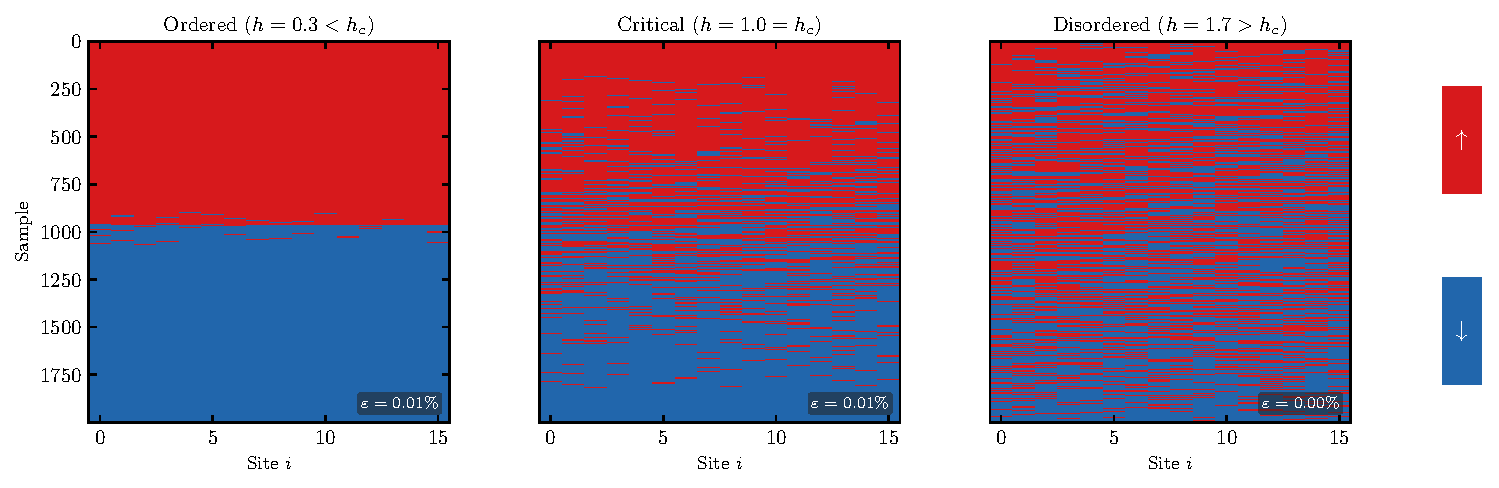
\includegraphics[width=0.82\linewidth]{../figures/spin_ordering_across_qpt.pdf}\\
\footnotesize samples from a trained model with 16 spins
\end{frame}

\section{Restricted Boltzmann Machines}

\begin{frame}{Introduction}
\begin{itemize}
    \item classical neural network with a layer of visible and hidden units~\cite{PhysRevResearch.2.023266,Carleo_2017,Gardas_2018}
\end{itemize}
\begin{block}{RBM energy function}
\begin{equation*}
E_{\boldsymbol\theta}(\mathbf{v},\mathbf{h})=\mathbf{a}\cdot \mathbf{v} -\mathbf{b}\cdot \mathbf{h} - \mathbf{h}\cdot \mathbf{W}^\top \cdot \mathbf{v}
\end{equation*}
\end{block}

\vfill
\centering
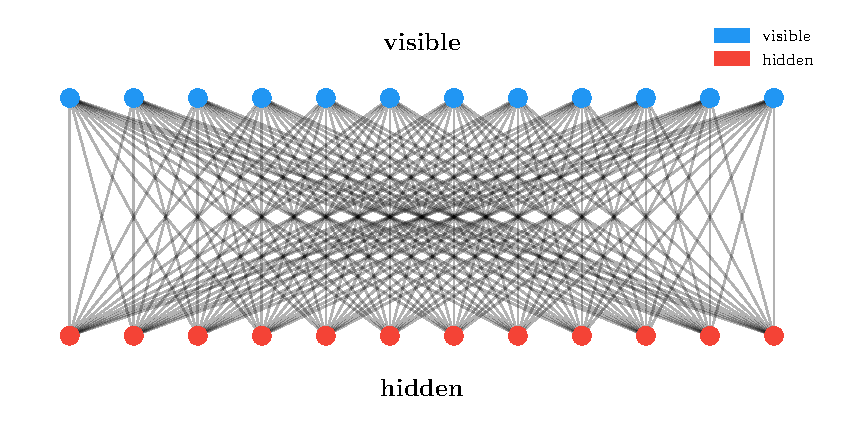
\includegraphics[width=0.5\linewidth]{../figures/rbm_abstract.pdf}\\
\footnotesize Fully connected RBM with 12 visible and 12 hidden units
\end{frame}

\begin{frame}{Training process 1}
\small
\begin{enumerate}
    \item Sampling from the Boltzmann distribution
\end{enumerate}
\begin{block}{RBM wavefunction: hidden units traced out}
\begin{equation*}
\ket{\Psi} = \sum_{\mathbf v} \Psi(\mathbf v)\ket{\mathbf v}, \qquad
\Psi(\mathbf{v})=\sqrt{\textstyle\sum_{\mathbf h} e^{-E_{\boldsymbol\theta}(\mathbf v,\mathbf h)}}
\end{equation*}
\begin{equation*}
\Longrightarrow\;\;
\Psi(\mathbf{v}) = e^{-\mathbf{a}\cdot \mathbf{v}/2} \prod_{j=1}^{N_h} \left[ 2\cosh\!\left(b_j + \textstyle\sum_i W_{ij} v_i\right) \right]^{1/2}
\end{equation*}
{\scriptsize closed form~\cite{Carleo_2017}}
\end{block}
\begin{block}{Born-rule marginal}
\begin{equation*}
    \rho(\mathbf{v})=\frac{|\Psi(\mathbf{v})|^2}{\sum_{\mathbf{v}'}|\Psi(\mathbf{v}')|^2}
\end{equation*}
\end{block}
\end{frame}

\begin{frame}{Training process 2}
\begin{enumerate}
\setcounter{enumi}{1}
    \item Calculating the local energies
    \begin{block}{Local energy~\cite{Gardas_2018}}
    \begin{equation*}
        E_\text{loc}(\mathbf v)=\frac{\langle \mathbf v|H|\Psi\rangle}{\Psi(\mathbf v)}
    \end{equation*}
    \end{block}
\end{enumerate}
\begin{block}{TFIM local energy~\cite{Gardas_2018,Carleo_2017}}
\begin{equation*}
    E_\text{loc}(\mathbf v) = -J\sum_{\langle i,j\rangle} v_i v_j - h\sum_i \frac{\Psi(\bar{\mathbf v}_i)}{\Psi(\mathbf v)}
\end{equation*}
\end{block}
\end{frame}

\begin{frame}{Training process 3}
\begin{enumerate}
\setcounter{enumi}{2}
    \item Calculate the log derivatives
    \begin{block}{Log-derivatives~\cite{Gardas_2018}}
    \footnotesize with $\phi_j = b_j + \sum_i W_{ij} v_i$
    \begin{equation*}
        \frac{\partial \log \Psi(\mathbf v)}{\partial \theta_k} = \frac{1}{2}
        \begin{cases}
        -v_i, & \theta_k = a_i\\
        \tanh(\phi_j), & \theta_k = b_j\\
        v_i \tanh(\phi_j), & \theta_k = W_{ij}
        \end{cases}
    \end{equation*}
    \end{block}
    \item Update the parameters using GD / Stochastic Reconfiguration
\end{enumerate}
\end{frame}

\section{Samplers}

\begin{frame}{Sampler Overview}
\begin{itemize}
    \item Classical Markov-Chain-Monte-Carlo samplers (Metropolis~\cite{Metropolis_1953,Hastings_1970}/Gibbs~\cite{Geman_1984}) on GPU and FPGA
    \item quantum samplers: D-Wave Quantum Annealer
\end{itemize}

\vfill
\centering
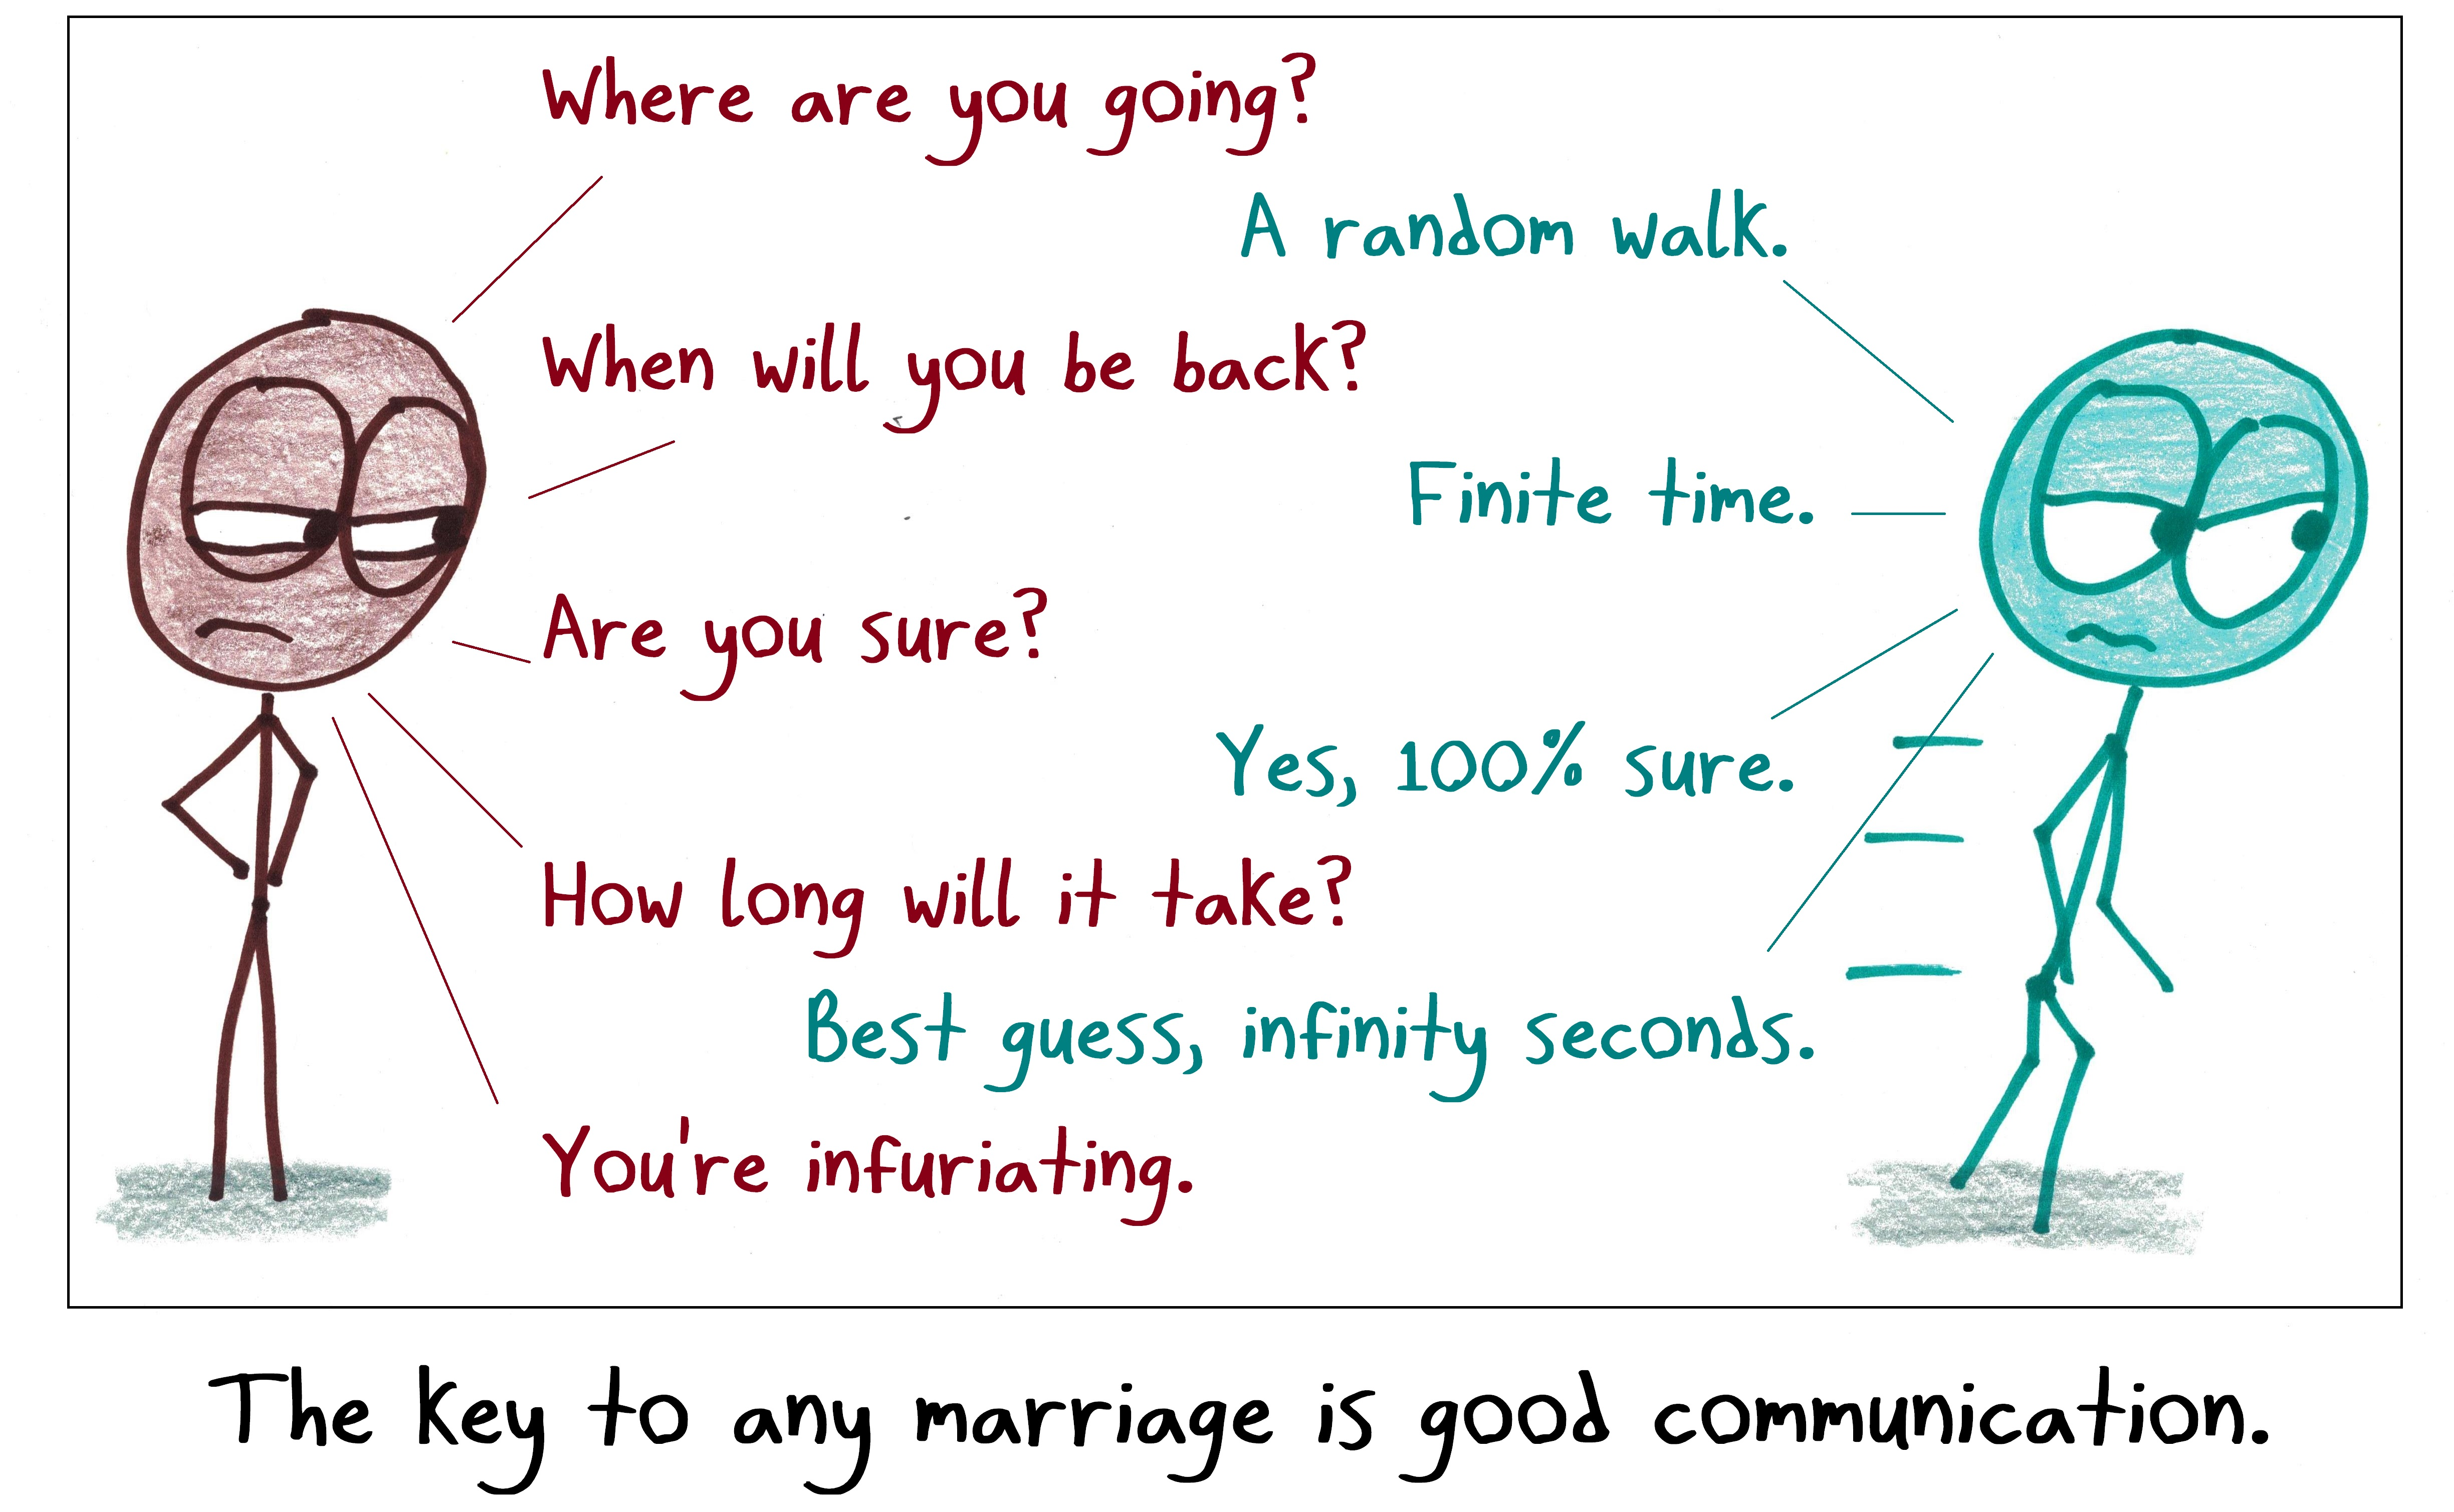
\includegraphics[width=0.48\linewidth]{figures/2018-5-28-random-walk.jpg}\\
{\scriptsize Ben Orlin, \textit{Math with Bad Drawings}, \url{https://mathwithbaddrawings.com/2018/10/31/im-going-on-a-random-walk/}}
\end{frame}

\begin{frame}{Temperature adjustment}
\begin{itemize}
    \item D-Wave sampler has unknown temperature
    \item CEM estimates the temperature from samples~\cite{kubo2025unlockingpowerboltzmannmachines}
\end{itemize}

\vfill
\begin{columns}[T,onlytextwidth]
\begin{column}{0.48\textwidth}
    \centering
    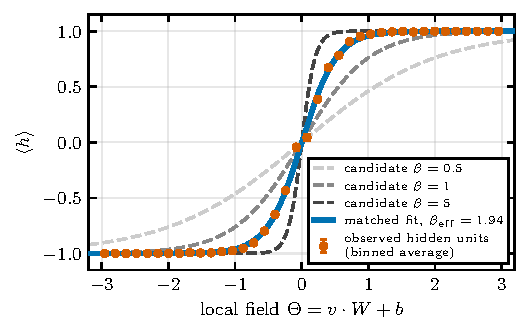
\includegraphics[width=\linewidth]{../figures/cem_matching_candidates.pdf}\\
    \footnotesize (a) Candidate fits vs.\ observed hidden units.
\end{column}
\begin{column}{0.48\textwidth}
    \centering
    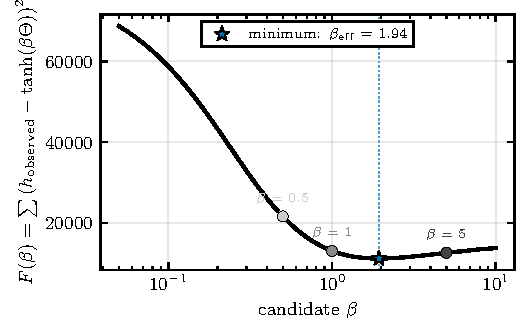
\includegraphics[width=\linewidth]{../figures/cem_matching_objective.pdf}\\
    \footnotesize (b) Matching objective $F(\beta)$.
\end{column}
\end{columns}
\end{frame}

\section{Results}

\begin{frame}{Methodology}
\begin{itemize}
    \item sample matched framework
    \item hyperparameter-matched comparison, TFIM ($h=0.5$), $N$ up to 64
\end{itemize}
\begin{block}{Error per spin}
\begin{equation*}
\varepsilon(t) = \frac{\bigl|\overline{E}_t - E_0\bigr|}{N}
\end{equation*}
\footnotesize $\overline{E}_t$: rolling-mean variational energy after cumulative sampling time $t$; $E_0$: exact ground-state energy
\end{block}
\begin{itemize}
    \item median and IQR over 20 seeds per solver and size
\end{itemize}
\end{frame}

\begin{frame}{Results: Error vs.\ Sampling Time}
\begin{columns}[c,onlytextwidth]
\begin{column}{0.64\textwidth}
\centering
\includegraphics[height=6.9cm]{../figures/error_vs_time_slide.pdf}
\end{column}
\begin{column}{0.34\textwidth}
\small
\begin{itemize}
    \item TFIM, $h=0.5$; horizontal line: $\varepsilon=0.1$
    \item $N=64$: Pegasus, FPGA and Zephyr cross $\varepsilon=0.1$ within a factor $\sim2$ ($0.47$, $0.59$, $0.84$\,s), IQR bands overlap
    \item Metropolis and SA cross more than $10\times$ later ($11.5$, $17.1$\,s)
\end{itemize}
\end{column}
\end{columns}
\end{frame}


\finalframe{Merci pour votre attention}


\begin{frame}[allowframebreaks]{References}
\footnotesize
\bibliography{../bib}
\end{frame}


\section*{Backup}

\begin{frame}{CEM \& Sampling Validation}
\begin{columns}[T,onlytextwidth]
\begin{column}{0.48\textwidth}
    \centering
    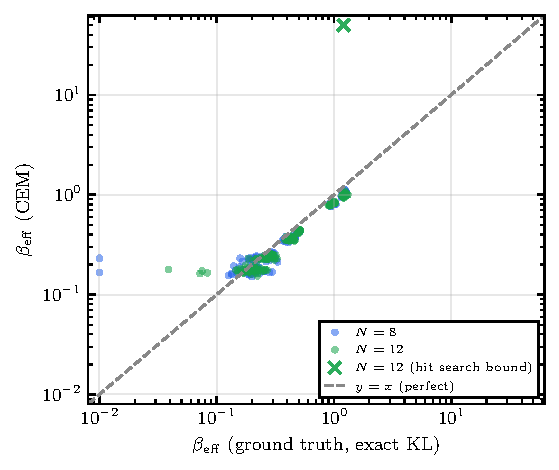
\includegraphics[height=3.1cm,keepaspectratio]{../figures/cem_validation_calibration.pdf}\\
    \footnotesize (a) CEM vs.\ exact ground truth
\end{column}
\begin{column}{0.48\textwidth}
    \centering
    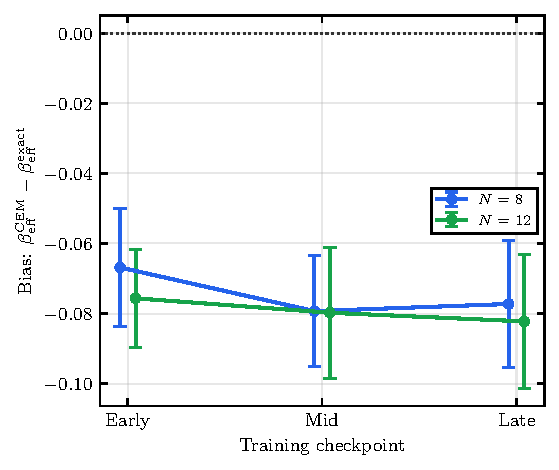
\includegraphics[height=3.1cm,keepaspectratio]{../figures/cem_validation_bias.pdf}\\
    \footnotesize (b) Bias across training
\end{column}
\end{columns}
\vspace{0.2cm}
\centering
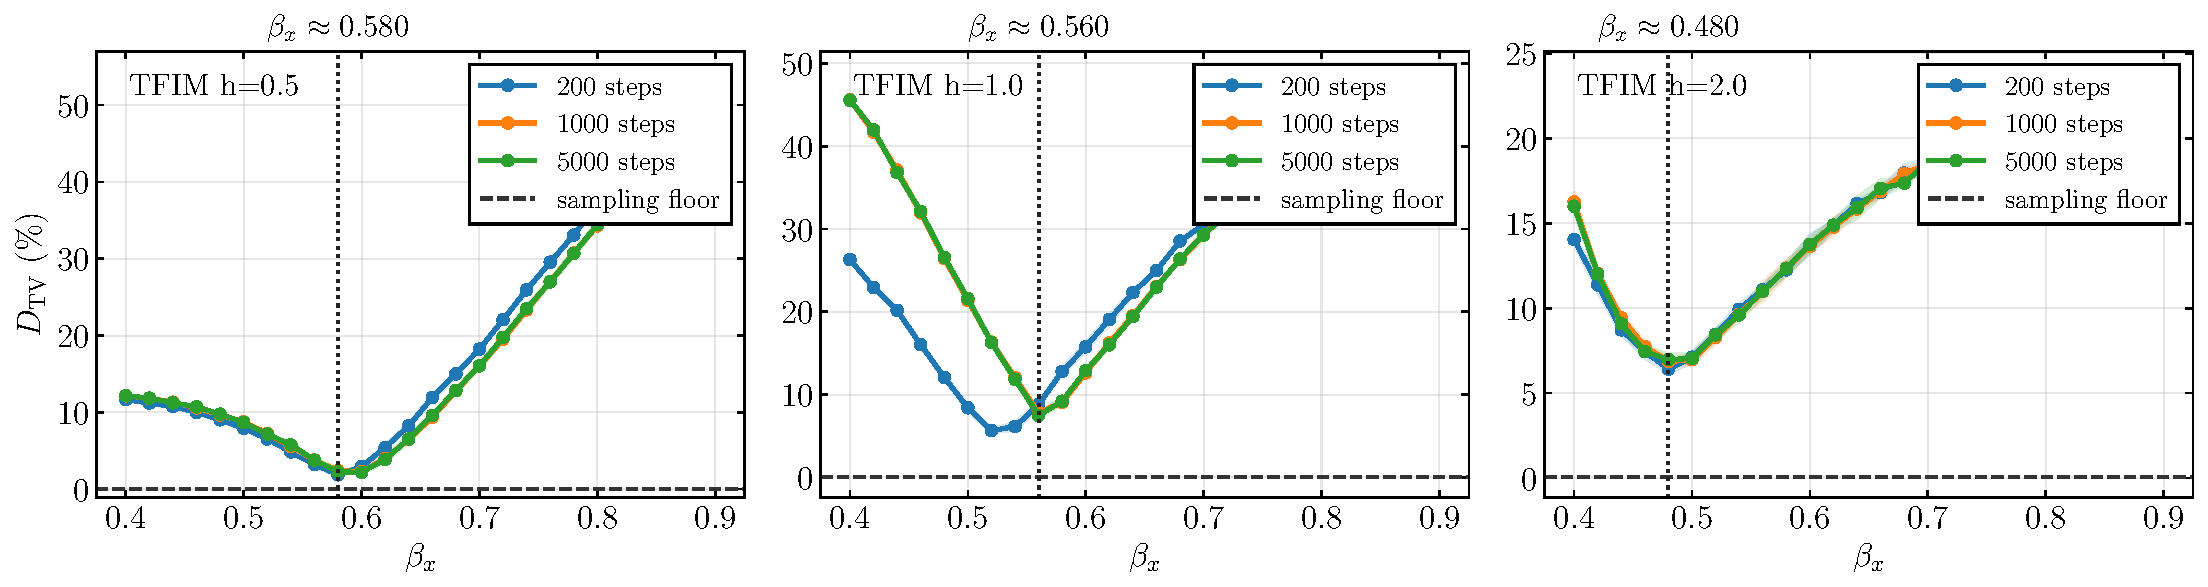
\includegraphics[height=2.7cm,keepaspectratio]{../figures/dtv_beta_scale_dtv_N8.pdf}\\
\footnotesize (c) $D_\mathrm{TV}$ vs.\ cooling sweeps
\end{frame}

\begin{frame}{Chain-free Embedding}
\begin{columns}[T,onlytextwidth]
\begin{column}{0.48\textwidth}
    \centering
    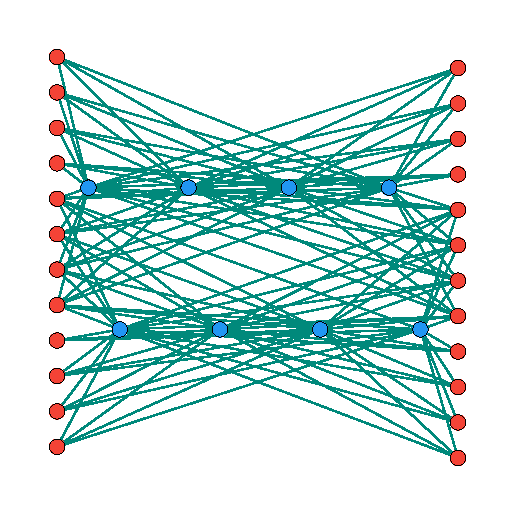
\includegraphics[height=5cm,keepaspectratio]{../figures/sparse_graph_construction/b.pdf}\\
    \footnotesize (a) Sparse RBM construction
\end{column}
\begin{column}{0.48\textwidth}
    \centering
    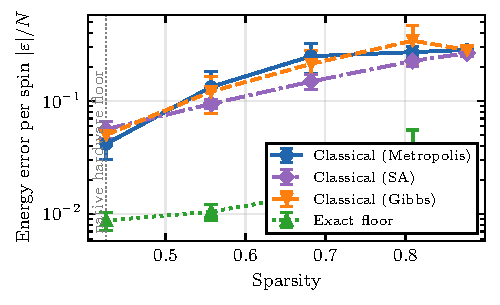
\includegraphics[height=4.3cm,keepaspectratio]{../figures/sparsity/sparsity_ablation_qpu_vs_classical.pdf}\\
    \footnotesize (b) Sparsity vs.\ sampler error
\end{column}
\end{columns}
\end{frame}

\begin{frame}{Parallel Embedding}
\begin{columns}[T,onlytextwidth]
\begin{column}{0.48\textwidth}
    \centering
    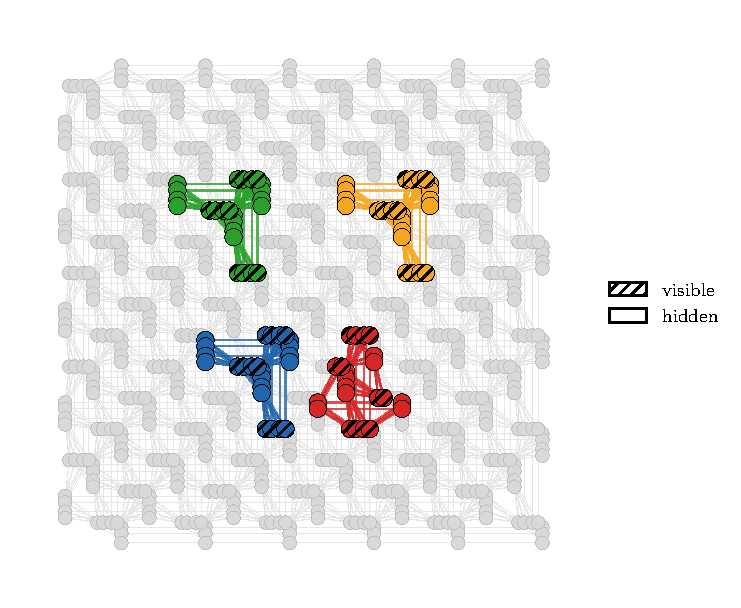
\includegraphics[width=\linewidth]{../figures/parallel_embedding/parallel_embedding_np4_pegasus.pdf}\\
    \footnotesize (a) Parallel embedding layout
\end{column}
\begin{column}{0.48\textwidth}
    \centering
    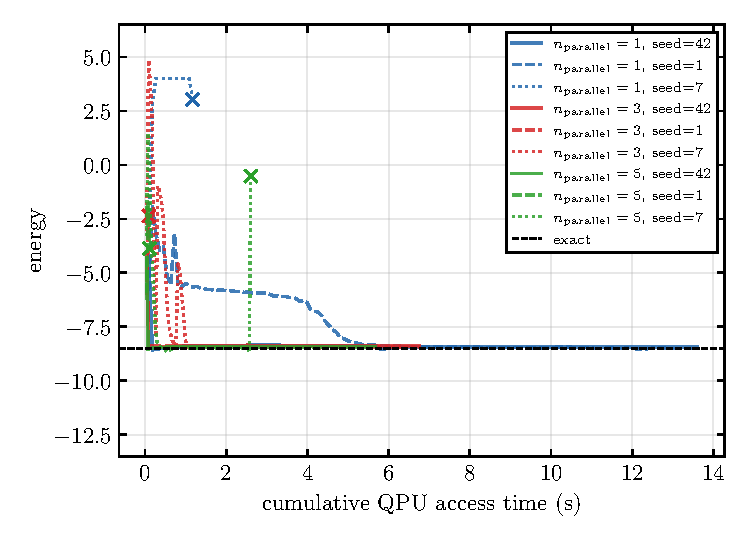
\includegraphics[width=\linewidth]{../figures/parallel_embedding/parallel_embedding_np_seeds_qpu_time.pdf}\\
    \footnotesize (b) QPU time speedup
\end{column}
\end{columns}
\end{frame}
\begin{frame}{Sign Problem: Stoquasticity}
\begin{block}{Stoquasticity}
A Hamiltonian is \emph{stoquastic} if, in the given basis, all off-diagonal elements are real and non-positive~\cite{2011772.2011773}.
\end{block}
\vspace{0.2cm}

Using $\sigma^x\ket{\uparrow}=\ket{\downarrow}$, $\sigma^y\ket{\uparrow}=i\ket{\downarrow}$, $\sigma^y\ket{\downarrow}=-i\ket{\uparrow}$, the Heisenberg exchange term acts on an antiparallel pair as
\begin{equation*}
\left(\sigma^x_i\sigma^x_j+\sigma^y_i\sigma^y_j\right)\ket{\uparrow\downarrow} = \ket{\downarrow\uparrow} + (i)(-i)\ket{\downarrow\uparrow} = 2\ket{\downarrow\uparrow}
\end{equation*}
Consequently, every antiparallel bond contributes
\begin{equation*}
\bra{\downarrow\uparrow}H_{ij}\ket{\uparrow\downarrow}=2J \;>\;0 \quad\Longrightarrow\quad \textbf{not stoquastic}
\end{equation*}
\end{frame}

\begin{frame}{Marshall Sign Rule}
\small
\begin{itemize}
    \item Bipartite lattice $A\cup B$: every nearest-neighbour ($J_1$) bond connects a site in $A$ to a site in $B$
    \item Unitary transformation, Pauli convention~\cite{Marshall_1955}:
    \begin{equation*}
    U = \prod_{i\in A}\sigma_i^z
    \end{equation*}
    \item Ground-state wavefunction after transformation (only positive amplitudes):
    \begin{equation*}
    U\ket{\psi_0} = \sum_\sigma |c_\sigma|\,\ket{\sigma}
    \end{equation*}
\end{itemize}

\vfill
\centering
\begin{columns}[T,onlytextwidth]
\begin{column}{0.48\textwidth}
\centering
\resizebox{\linewidth}{!}{%
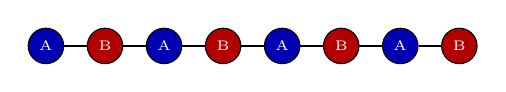
\begin{tikzpicture}[every node/.style={circle,draw,minimum size=4.5mm,inner sep=0pt,font=\tiny}]
\foreach \i/\c/\lab in {0/blue!70!black/A,1/red!70!black/B,2/blue!70!black/A,3/red!70!black/B,4/blue!70!black/A,5/red!70!black/B,6/blue!70!black/A,7/red!70!black/B} {
  \node[fill=\c,text=white] (s\i) at (\i*0.75,0) {\lab};
}
\foreach \i in {0,1,2,3,4,5,6} {
  \pgfmathtruncatemacro{\j}{\i+1}
  \draw[thick] (s\i) -- (s\j);
}
\end{tikzpicture}}\\
\footnotesize (a) $J_1$: always $A$--$B$
\end{column}
\begin{column}{0.48\textwidth}
\centering
\resizebox{\linewidth}{!}{%
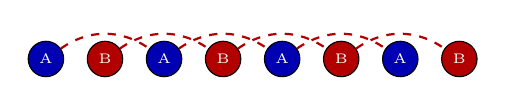
\begin{tikzpicture}[every node/.style={circle,draw,minimum size=4.5mm,inner sep=0pt,font=\tiny}]
\foreach \i/\c/\lab in {0/blue!70!black/A,1/red!70!black/B,2/blue!70!black/A,3/red!70!black/B,4/blue!70!black/A,5/red!70!black/B,6/blue!70!black/A,7/red!70!black/B} {
  \node[fill=\c,text=white] (t\i) at (\i*0.75,0) {\lab};
}
\foreach \i in {0,1,2,3,4,5} {
  \pgfmathtruncatemacro{\j}{\i+2}
  \draw[thick,dashed,red!70!black] (t\i) to[bend left=35] (t\j);
}
\end{tikzpicture}}\\
\footnotesize (b) $J_2$: same sublattice $\to$ breaks bipartiteness
\end{column}
\end{columns}
{\scriptsize Marshall correction survives moderate frustration~\cite{Richter_1994,Voigt_2000}}
\end{frame}

\begin{frame}{Marshall Sign Correction}
\centering
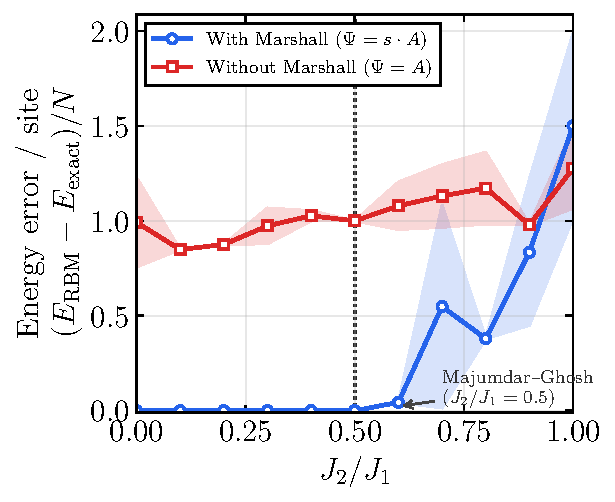
\includegraphics[width=0.75\linewidth]{../figures/marshall_comparison/marshall_comparison_energy.pdf}\\
\footnotesize Energy error per site vs.\ $J_2/J_1$, with/without correction
\end{frame}

\begin{frame}{RBM Convergence Curves}
\centering
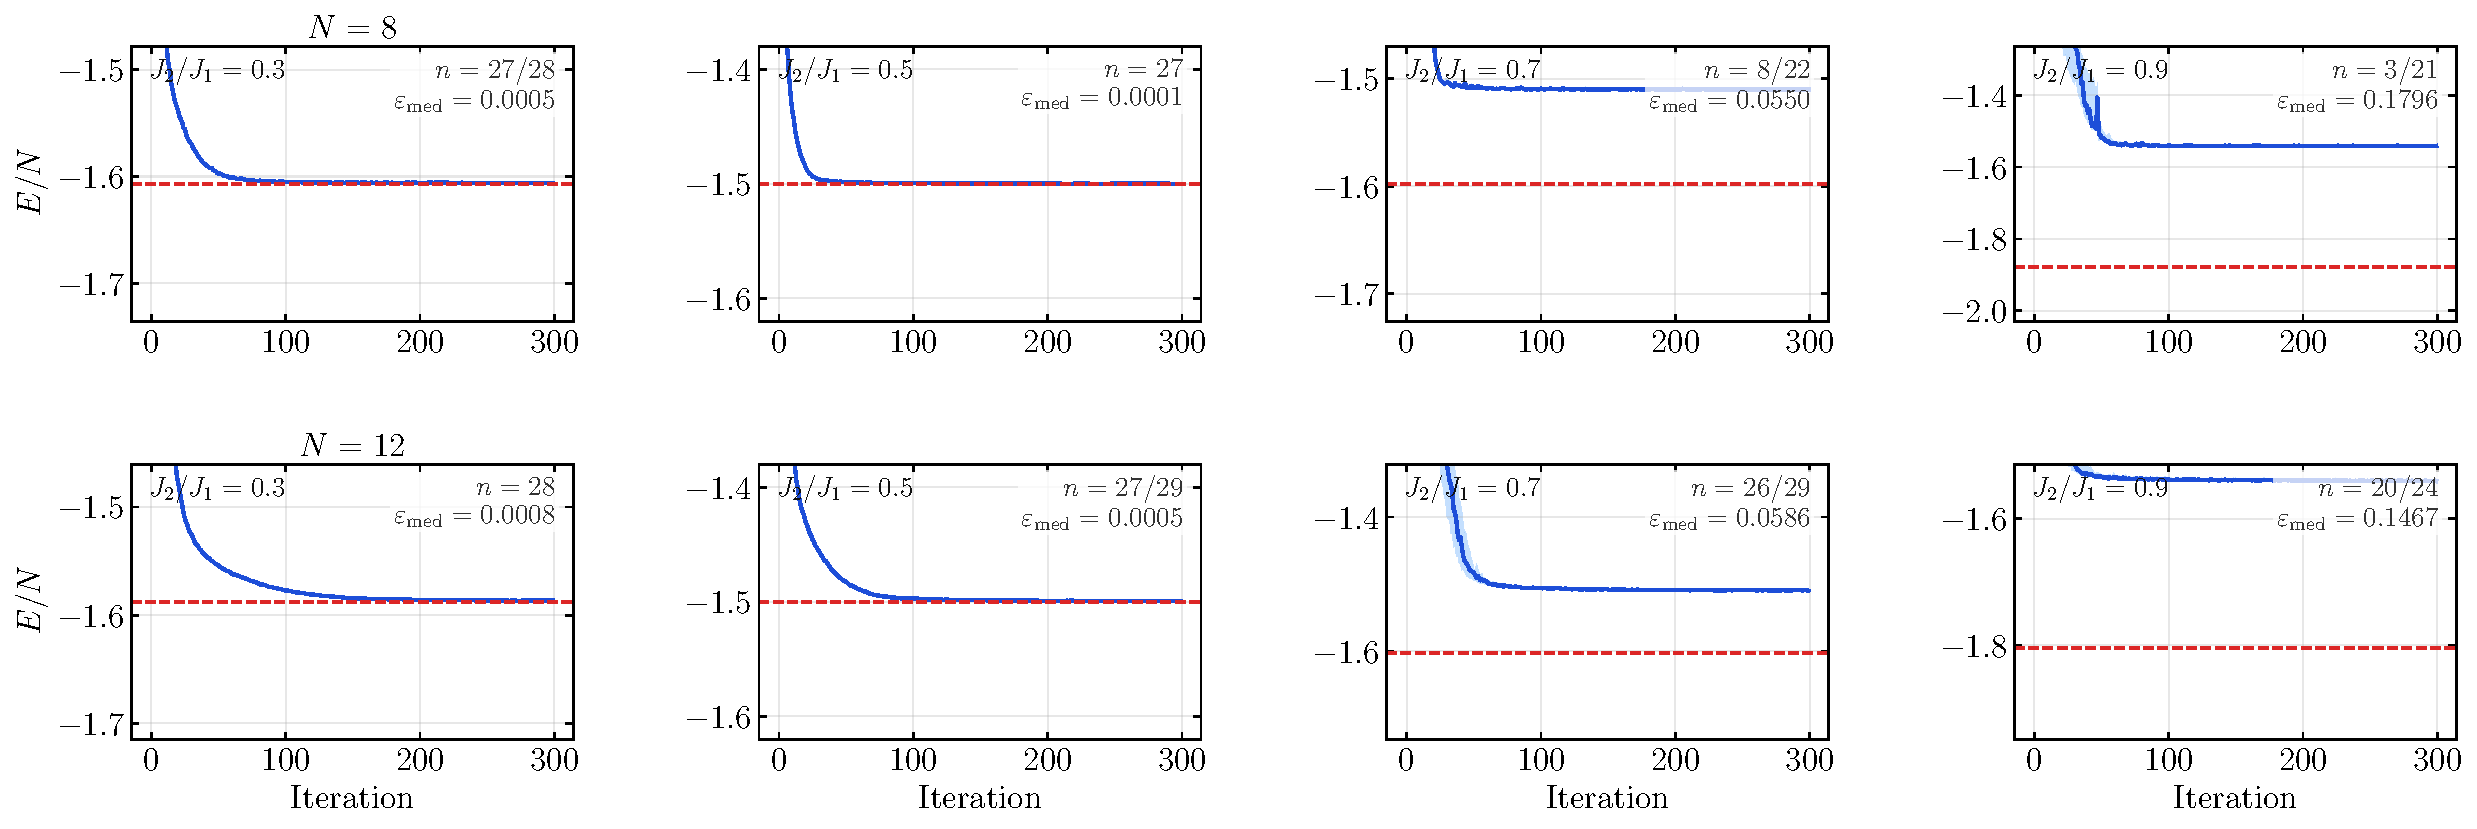
\includegraphics[width=\linewidth]{../figures/fig_convergence_median.pdf}\\
\footnotesize $E/N$ vs.\ SR iteration, frustrated Heisenberg chain
\end{frame}

\end{document}
